\documentclass{article}
\usepackage[utf8]{inputenc}
%\usepackage{hyperref}
\usepackage[english]{babel}
\usepackage{color}
\usepackage[colorinlistoftodos]{todonotes}
\usepackage{amsmath,amssymb,amsfonts}
\usepackage{amsthm}
\usepackage{enumerate}
\usepackage{enumitem}
\usepackage{array}
\usepackage{multicol}
\usepackage[numbered,framed]{matlab-prettifier}
\usepackage[font={color=black,bf},figurename=Fig.,labelfont={it}]{caption}
\usepackage{parskip}
\usepackage{subfiles}
\usepackage[toc,page]{appendix}
\usepackage{graphicx}
\usepackage{tocloft}
\usepackage{titlepic}
\usepackage{wrapfig}
\usepackage{float}
\usepackage{cite}
\usepackage[utf8]{inputenc}
\usepackage{tabu}
\usepackage{amsfonts}
\usepackage{listings}
\usepackage{tikz}
\usetikzlibrary{matrix,calc}
\usepackage[nottoc]{tocbibind}
\usepackage{filecontents}
\usepackage{textcomp}
\usepackage{xcolor}
\usepackage{epstopdf}
\usepackage{caption}
\usepackage{booktabs}
\usepackage{gensymb}
\usepackage[compact]{titlesec}
\usepackage{fancyvrb}
\usepackage{eurosym}
\usepackage{soul}
\usepackage{longtable}
\usepackage[margin=1in]{geometry}
\pagestyle{plain}
%\usepackage[a4paper, total={7in, 10in}]{geometry}  Dit is voor mee text p.pag
\usepackage{hyperref}
\usepackage{import}
\usepackage[utf8]{inputenc}
\usepackage{subcaption}
\definecolor{mygreen}{RGB}{28,172,0} 
\definecolor{mylilas}{RGB}{170,55,241}
\usepackage{subcaption}
\usepackage{lscape}
\usepackage{svg}
\usepackage{multirow}
\usepackage[absolute,overlay]{textpos}
\newtheorem{theorem}{Theorem}
\newtheorem{definition}{Definition}
\newtheorem{example}{Example}
\setcounter{MaxMatrixCols}{13}
\newcommand{\doctitle}{Multi-observer for control}
\newcommand{\docsubtitle}{Bachelor End Project}
\newcommand{\me}{Julian Gootzen}
\newcommand{\version}{Draft version}
\newcommand{\placeMonthYear}{Eindhoven, January 2025}
\newcommand{\department}{Department of Mechanical Engineering}
\newcommand{\group}{Dynamics and control}
\newcommand{\firstCommitteeMember}{Michelle Chong} % use all the titles for 

\newcommand{\cJ}{|\mathcal{J}|}
\newcommand{\cP}{|\mathcal{P}|}
\newcommand{\pamu}{\texttt{pm}}
\newcommand{\mcJ}{\mathcal{J}}
\newcommand{\mcP}{\mathcal{P}}
\newcommand{\mcO}{\mathcal{O}}
\newcommand{\B}{\mathcal{B}}
\newcommand{\A}{\mathcal{A}}

% matlab parula colors
\definecolor{parula1}{rgb}{0.2422, 0.1504, 0.6603}
\definecolor{parula2}{rgb}{0.2021, 0.4788, 0.9911}
\definecolor{parula3}{rgb}{0.0704, 0.7457, 0.7258}
\definecolor{parula4}{rgb}{0.9184, 0.7308, 0.3890}
\definecolor{parula5}{rgb}{0.9769,    0.9839,    0.2805}


\begin{document}
\lstset{language=Matlab,
	basicstyle = \scriptsize,
    breaklines=true,
    morekeywords={matlab2tikz},
    keywordstyle=\color{blue},
    morekeywords=[2]{1}, keywordstyle=[2]{\color{black}},
    identifierstyle=\color{black},
    stringstyle=\color{mylilas},
    commentstyle=\color{mygreen},
    showstringspaces=false,
    numbers=left,
    numberstyle={\small \color{black}},
    numbersep=9pt, 
    emph=[1]{for,end,break},emphstyle=[1]\color{red},   
}


\title{}
\author{ \hfill }

\input{report/General/Titlepage.tex}
%\maketitle\thispagestyle{empty}

\newpage
\tableofcontents\thispagestyle{empty}

%\section{Introduction}
%\subsection{dit is een ondertitel}
%\subsubsection{Dit is een onder-ondertitel}

\newpage
\section{Problem Statement}
In the modern world large-scale systems such as power grids, transportation systems, and industrial processes are increasingly autonomous and interconnected. These systems make decisions based on real-time data, collected by sensors. For large systems, which require a lot of variables to describe the state, measuring all of these variables can be expensive or impractical. In these situations an \textit{observer} can be used to reconstruct the full state of the system from a subset of the \textit{state variables} \cite[Section 16.5]{Hespanha2018LinearTheory}. Unfortunately, these systems are vulnerable to faulty sensor input. The system will then make decisions based on this false data and possibly cause failures or equipment damage. In a power grid this could lead to large-scale blackouts. \textcolor{red}{cite this entire thing} \\

The sensor data being erroneous could, for example, be caused by damage to the sensor or a malicious actor interfering with the sensor. This report will focus on the second case: a number of sensors in our system have been taken over by attackers. The attacker has full control over the sensor output signal and it can be any, potentially unbounded, value. Secure state estimation is the problem of providing an accurate state estimation when sensors are subject to the aforementioned malicious attacks.


\textcolor{red}{find other approaches}


This BEP aims to provide a comparison between two methods that aim to address the secure state estimation problem: the conventional multi-observer (CMO)\cite{Chong2015ObservabilityAttacks} and the state-sharing multi-observer (SSMO)\cite{Chong2023MemoryAlgorithms}. The SSMO aims to overcome the bottleneck of the CMO: memory-usage. The memory required to operate a CMO scales unfavourably with the number of outputs. The SSMO aims to provide a more scalable solution to secure state estimation problem. A mass-spring-damper system will be used to study the performance of both the CMO and SSMO.





\newpage
\section{System definition}\label{ch:system-definition}
Let us define the following continuous, nonlinear, time invariant, multiple-input multiple-output system: 
\begin{equation}\label{eqn:standard-system}
    \begin{split}
        \dot{x}(t) &= Ax(t) + Bu(t) + E\phi(x) \\
        y_i(t) &= C_ix(t) + Du(t) + v_i(t) + \tau_i(t) \quad i \in \mathcal{N} = \{1,2,\dots,N_O\}.
    \end{split}
\end{equation}
Where $x \in \mathbb{R}^{n_x}$, $y \in \mathbb{R}^{n_y}$, $u \in \mathbb{R}^{n_u}$ and the nonlinearity $\phi(x) \in \mathbb{R}^{n_{\phi}}$. Each $i$ indicates a single output, so each $y_i$ corresponds to a $C_i \in \mathbb{R}^{1 \times n_x}$. The variables without subscript $y$ and $C$, denote all $y_i$ and $C_i$ stacked on top of each other 
$y = 
\begin{bmatrix}
    y_1 & y_2 & \cdots & y_{N} \\
\end{bmatrix}^{T}$ and
$C =
\begin{bmatrix}
    C_1^T & C_2^T & \cdots & C_N^T \\
\end{bmatrix}^{T}$
Let us consider the scenario where an attacker attacks a number of outputs $y_i$, where the attacker then has full control over the attack signal $\tau_i$. No assumptions are made about $\tau_i$, it can be any unbounded signal. Let us denote the set of attacked outputs as 
\begin{equation}\label{eqn:M-definition}
    \mathcal{M} \subset \mathcal{N}.
\end{equation}
Figure \ref{fig:attack-diagram} shows an example where $\mathcal{N}=\{1,2,3,4,5\}$ and $\mathcal{M} = \{2,5\}$.

\begin{figure}[ht]
    \centering
    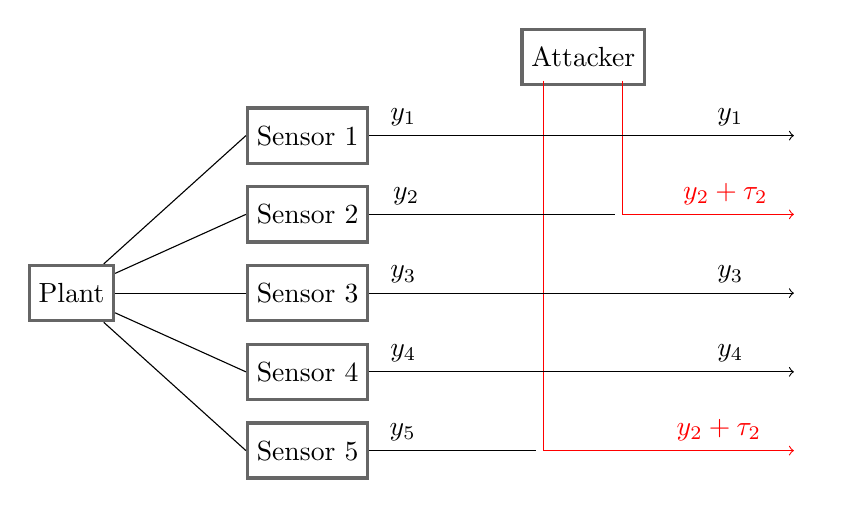
\begin{tikzpicture}[
        sensor/.style={rectangle, draw=black!60, very thick, minimum size=7mm},
        ]
        \node (obin1) at (9.3,2) {};
        \node (obin2) at (9.3,1) {};
        \node (obin3) at (9.3,0) {};
        \node (obin4) at (9.3,-1) {};
        \node (obin5) at (9.3,-2) {};
        
        \node (attacker) at (6.5,3) [sensor] {Attacker};
        \node (a1s2) at (7,1) {};

        \draw[->,red] (7,2.7) -- (7,1) -- node[pos=0.6,above] {$y_2+\tau_2$} (obin2);
        \draw[->,red] (6,2.7) -- (6,-2) -- node[pos=0.7,above] {$y_2+\tau_2$} (obin5);
    
        
        \node (sensor3) at (3,0) [sensor] {Sensor 3}
            edge [->] node[pos=0.08,above] {$y_3$} node[pos=0.85,above] {$y_3$} (obin3);
        \node (sensor2) at (3,1) [sensor] {Sensor 2}
            edge [-] node[pos=0.15,above] {$y_2$} (6.9,1);
        \node (sensor1) at (3,2) [sensor] {Sensor 1}
            edge [->] node[pos=0.08,above] {$y_1$} node[pos=0.85,above] {$y_1$} (obin1);
        \node (sensor4) at (3,-1) [sensor] {Sensor 4}
            edge [->] node[pos=0.08,above] {$y_4$} node[pos=0.85,above] {$y_4$} (obin4);
        \node (sensor5) at (3,-2) [sensor] {Sensor 5}
            edge [-] node[pos=0.2,above] {$y_5$} (5.9,-2);
        \node (plant) at (0,0) [sensor] {Plant}
            edge [-] (sensor1.west)
            edge [-] (sensor2.west)
            edge [-] (sensor3.west)
            edge [-] (sensor4.west)
            edge [-] (sensor5.west);
        
    \end{tikzpicture}
    \caption{A system with 2 out of 5 outputs attacked}
    \label{fig:attack-diagram}
\end{figure}


\subsection{Case study: multi-mass-spring-damper system}
Let us now introduce the system that will be used as a case study: a mass-spring-damper system. This system consists of $b$ mass-spring-dampers in series. Where $x_a \in \mathbb{R},a=1,2,\dots,b$ denotes the relative position with respect to the previous mass. So the absolute position of a block with respect to the fixed-world is
\begin{equation}\label{eqn:mass-position-wrt-fixed-world}
    \sum^{a}_{j=1}x_j.
\end{equation}
The other variables denote the following: $k_a\in \mathbb{R}>0$ is the linear spring constant, $\eta_a\in \mathbb{R}>0$ is the nonlinear spring constant, $c_a\in \mathbb{R}\geq0$ is the damping constant and $F_a$ is a force acting on the mass.
\begin{figure}[H]
    \centering
    \includegraphics[width=0.9\linewidth]{report/Figures/Mass-spring-damper system.png}
    \caption{Multi-mass-spring-damper system for $b$ mass-spring-dampers in series.}
    \label{fig:mass-spring-damper-system-series}
\end{figure}

We will now derive the state-space form of the system as drawn in Figure \ref{fig:mass-spring-damper-system-series}. We will start by deriving the equation of motion for the first $b-1$ masses. The sum of forces on a single mass is
\begin{equation}\label{eqn:free-body-equation}
    m_a\ddot{x}_a = F_a - F_s(x_a,k_a,\zeta_a) - F_d(\dot{x}_a,c_a) + F_s(x_{a+1},k_{a+1},\zeta_{a+1}) + F_d(\dot{x}_{a+1},c_{a+1}).
\end{equation}
Let us now define the spring and damping forces $F_s(x_a,k_a,\zeta_a)$ and $F_d(\dot{x}_a,c_a)$ respectively
\begin{equation*}
    F_s(x_a,k_a,\zeta_a) = k_ax_a + k_a \zeta_a^2 x_a^3, \quad F_d(\dot{x}_a,c_a) = c_a\dot{x}_a.
\end{equation*}
The formula for the nonlinear spring force is taken from the hardening spring example in \cite[Section 1.2.3]{Khalil2002NonlinearSystems}, the damping force is linear. The expressions for the spring force and damping force will be written as $F_s(x_a)$ and $F_d(\dot{x}_a)$ respectively, where the constants $k_a$, $\eta_a$ and $c_a$ are implicitly passed to the function. $F_s$ will be separated into a linear and nonlinear part as
\begin{equation}\label{eqn:nonlinear-spring}
    \begin{split}
        F_s(x_a) &= F_s^L(x_a) + F_s^{NL}(x_a) \\
        F_s^L(x_a) &= k_ax_a \quad , F_s^{NL}(x_a) = k_a\zeta_a^2x^3_a
    \end{split}    
\end{equation}

We will now apply Equation \eqref{eqn:free-body-equation} on the first mass, using the split up $F_s$ as in Equation \eqref{eqn:nonlinear-spring}

\begin{equation*}
    m_1\Ddot{x}_1 = u_1 - k_1x_1 - c_1\dot{x}_1 + k_2x_2 + c_2\dot{x}_2 - F_s^{NL}(x_1) + F_s^{NL}(x_2), \quad u_1 = F_1,
\end{equation*}
which can be rewritten into
\begin{equation}\label{eqn:mass-spring-damper-first-mass-eom}
    \Ddot{x}_1 = -\frac{k_1}{m_1}x_1 -\frac{c_1}{m_1}\dot{x}_1 + \frac{k_2}{m_1}x_2 + \frac{c_2}{m_1}\dot{x}_2 + \frac{u_1}{m_1} - \frac{F_s^{NL}(x_1)}{m_1} + \frac{F_s^{NL}(x_2)}{m_1}.
\end{equation}
Doing this for the second mass gives the following result:
\begin{equation*}
    \Ddot{x}_2 = -\frac{k_2}{m_2}x_2 - \frac{c_2}{m_2}\dot{x}_2 + \frac{k_3}{m_2}x_3 + \frac{c_3}{m_2}\dot{x}_3 + \frac{u_2}{m_2} - \frac{F_s^{NL}(x_2)}{m_1} + \frac{F_s^{NL}(x_3)}{m_1}.
\end{equation*}
which can be generalised into
\begin{equation}\label{eqn:mass-spring-damper-centre-mass-eom}
    \Ddot{x}_a =  -\frac{k_a}{m_a}x_a - \frac{c_a}{m_a}\dot{x}_a + \frac{k_{a+1}}{m_a}x_{a+1} + \frac{c_{a+1}}{m_a}\dot{x}_{a+1} + \frac{u_a}{m_a} - \frac{F_s^{NL}(x_a)}{m_a} + \frac{F_s^{NL}(x_{a+1})}{m_a}.
\end{equation}
which holds for $a \in \{2,3,\dots,b-2,b-1\}$. Now only the last mass remains
\begin{equation}\label{eqn:mass-spring-damper-last-mass-eom}
    \Ddot{x}_b = -\frac{k_b}{m_b}x_b - \frac{c_b}{m_b}\dot{x}_b + \frac{u_b}{m_b} - \frac{F_s^{NL}(x_b)}{m_b}
\end{equation}

Let us now define the state vector $x$ as in Equation \eqref{eqn:standard-system} as
\begin{equation}\label{eqn:msd-x}
    x =
    \begin{bmatrix}
        x_1 & \dot{x}_1 & x_2 & \dot{x}_2 & \cdots & x_b & \dot{x}_{b}
    \end{bmatrix}^T
\end{equation}
Using equations \eqref{eqn:mass-spring-damper-first-mass-eom}\eqref{eqn:mass-spring-damper-centre-mass-eom}\eqref{eqn:mass-spring-damper-last-mass-eom} can now be used to construct the $A$ and $B$ matrices in equation \eqref{eqn:standard-system}
\begin{equation}\label{eqn:msd-A}
    A =
    \begin{bmatrix}
        0 & 1 & 0 & 0 & 0 & 0 & \cdots & 0 & 0 & 0 & 0 \\
        -\frac{k_1}{m_1} & -\frac{c_1}{m_1} & \frac{k_2}{m_1} & \frac{c_2}{m_1} & 0 & 0 & \cdots & 0 & 0 & 0 & 0 \\
        0 & 0 & 0 & 1 & 0 & 0 & \cdots & 0 & 0 & 0 & 0 \\
       0 & 0 & -\frac{k_2}{m_2} & -\frac{c_2}{m_2} & \frac{k_3}{m_2} & \frac{c_3}{m_2} & \cdots & 0 & 0 & 0 & 0 \\
        \vdots & \vdots & \vdots & \vdots & \vdots & \vdots & \ddots & \vdots & \vdots & \vdots & \vdots \\
        0 & 0 & 0 & 0 & 0 & 0 & \cdots & 0 & 0 & 0 & 1 \\
        0 & 0 & 0 & 0 & 0 & 0 & \cdots & 0 & 0 & -\frac{k_b}{m_b} & -\frac{c_b}{m_b} \\
    \end{bmatrix}
\end{equation}
and
\begin{equation}\label{eqn:msd-B}
    B = 
    \begin{bmatrix}
        0 & 0 & \cdots & 0 \\
        \frac{1}{m_1} & 0 & \cdots & 0 \\
        0 & 0 & \cdots & 0 \\
        0 & \frac{1}{m_2} & \cdots & 0 \\
        \vdots & \vdots & \ddots & \vdots \\
        0 & 0 & \cdots & 0 \\
        0 & 0 & \cdots & \frac{1}{m_b} \\
    \end{bmatrix}.
\end{equation}
Let us now derive the nonlinear contributions $\phi$ and $E$ from equation \eqref{eqn:standard-system} and from equations \eqref{eqn:mass-spring-damper-first-mass-eom},\eqref{eqn:mass-spring-damper-centre-mass-eom},\eqref{eqn:mass-spring-damper-last-mass-eom}. First we need to define the intermediary matrix
\begin{equation}\label{eqn:Hx}
    H_{x} =
    \begin{bmatrix}
        1 & 0 & 0 & 0 & \cdots & 0 & 0 & 0 & 0 \\
        0 & 0 & 1 & 0 & \cdots & 0 & 0 & 0 & 0 \\
        \vdots & \vdots & \vdots & \vdots & \ddots & \vdots & \vdots & \vdots & \vdots \\
        0 & 0 & 0 & 0 & \cdots & 1 & 0 & 0 & 0 \\
        0 & 0 & 0 & 0 & \cdots & 0 & 0 & 1 & 0 \\
    \end{bmatrix}_{n_{\phi} \times n_{x}},
\end{equation}
which extracts the first $n_{\phi}$ relative positions from $x$ performing the multiplication $Hx$ and where $n_{\phi}$ denotes the 'size' of the nonlinearity. Performing the function $\phi$ on a vector implies performing $F^{NL}_s$ on every element
\begin{equation}
    \phi(H_{x}x) =
    \begin{bmatrix}
        F_s^{NL}(x_1) & F_s^{NL}(x_2) & \cdots & F_s^{NL}(x_{n_{\phi}})
    \end{bmatrix}_{1 \times n_{\phi}}^T
\end{equation}
and
\begin{equation}\label{eqn:msd-E}
    E =
    \begin{bmatrix}
        0 & 0 & 0 & \cdots & 0 \\
        -\frac{1}{m_1} & \frac{1}{m_1} & 0 & \cdots & 0 \\
        0 & 0 & 0 & \cdots & 0 \\
        0 & -\frac{1}{m_2} & \frac{1}{m_2} & \cdots & 0 \\
        \vdots & \vdots & \vdots & \ddots & \vdots \\
        0 & 0 & 0 & \cdots & 0 \\
        0 & 0 & 0 & \cdots & -\frac{1}{m_b} \\
    \end{bmatrix}_{n_x \times n_{\phi}}
\end{equation}
can be defined. We will now construct the $C$ matrix, in order to do so let us note that only the absolute positions \eqref{eqn:mass-position-wrt-fixed-world} of each mass are measured. This leads to
\begin{equation}\label{eqn:msd-C}
    C = 
    \begin{bmatrix}
        1 & 0 & 0 & 0 & \cdots & 0 & 0 & 0 & 0 \\
        1 & 0 & 1 & 0 & \cdots & 0 & 0 & 0 & 0 \\
        \vdots & \vdots & \vdots & \vdots & \ddots & \vdots & \vdots & \vdots & \vdots \\
        1 & 0 & 1 & 0 & \cdots & 1 & 0 & 0 & 0 \\
        1 & 0 & 1 & 0 & \cdots & 1 & 0 & 1 & 0 \\
    \end{bmatrix}
\end{equation}
where each row is a single output. In system as in Figure \ref{fig:mass-spring-damper-system-series} the $D$ matrix is equal to $0$.
\begin{example}\label{ex:system}
    Let us define a linear system with two masses and the properties: $m_i=1 \text{[kg]}, k_i=15\text{[N/m]}$ and $c_i=2 \text{[Ns/m]}$ for $i=1,2$. We now construct the system matrices as
    \begin{equation}\label{eqn:example-system}
    A =
    \begin{bmatrix}
        0 & 1 & 0 & 0 \\
        -15 & -2 & 15 & 2 \\
        0 & 0 & 0 & 1 \\
        0 & 0 & -15 & -2 \\
    \end{bmatrix}, \quad
    B = 
    \begin{bmatrix}
        0 & 0 \\
        1 & 0 \\
        0 & 0 \\
        0 & 1 \\
    \end{bmatrix}, \quad
    C =
    \begin{bmatrix}
        1 & 0 & 0 & 0 \\
        1 & 0 & 1 & 0 \\
    \end{bmatrix}, \quad
    D = 0.
    \end{equation}
\end{example}
\newpage
\section{State estimation}\label{ch:state-estimation}
This chapter first discussed the motivation for full state estimation. It also introduces the concept of observability and how it relates to state estimation. A standard 'single-observer' will be derived for linear systems and it will be expanded to also observe system with a non-linearity.


\subsection{Motivation for full state estimation}
Let us first discuss why there is a need for state estimation, consider the continious linear time invariant system
\begin{equation}\label{eqn:standard-noiseless-system}
    \dot{x}(t) = Ax(t) + Bu(t), \quad y(t) = Cx(t) + Du(t).
\end{equation}
The solution to this system can be written as
\begin{equation*}
    \begin{split}
        x(t) &= e^{tA}x_{0} + \int_{0}^{t}e^{(t-\tau)A}Bu(\tau)d\tau \\
        y(t) &= Ce^{tA}x_{0} + \int_{0}^{t}Ce^{(t-\tau)A}Bu(\tau)d\tau + Du(t).
    \end{split}
\end{equation*}
where $x_0 = x(0)$ \cite[Eqn. 6.4]{Hespanha2018LinearTheory}. When there is no input, i.e. $u(t)=0$ for $t \geq 0$, system \eqref{eqn:standard-noiseless-system} reduces to
\begin{equation*}
    \dot{x}(t) = Ax(t), \quad y(t) = Cx(t)
\end{equation*}
which has the solution
\begin{equation}\label{eqn:zero-input-solution}
    x(t) = e^{tA}x_0, \quad y(t) = Ce^{tA}x_0.
\end{equation}
Let us now consider the definition of Lyapunov stability as in \cite[Th. 8.2]{Hespanha2018LinearTheory}, which states that a system is stable if and only if all the eigenvalues $\lambda_i,i=1,2,\dots,n$ of $A$ have strictly negative real parts. The matrix exponential in equation \eqref{eqn:zero-input-solution} computed by writing the matrix $A$ into its Jordan normal form $J=PAP^{-1}$, where $P$ is a change of basis matrix. The solution can then be written as 
\begin{equation}\label{eqn:jordan-form-exponential}
    x(t) = P^{-1}e^{tJ}Px_0
\end{equation}
\cite[Section 7.3]{Hespanha2018LinearTheory}. The matrix $J$ takes the following form
\begin{equation}\label{eqn:jordan-matrix}
    J =
    \begin{bmatrix}
        J_1 & 0 & \cdots & 0 \\
        0 & J_2 & \cdots & 0 \\
        \vdots & \vdots & \ddots & \vdots \\
        0 & 0 & \cdots & J_l \\
    \end{bmatrix}
\end{equation}
where each $J_i$ is a Jordan block that has the form
\begin{equation}\label{eqn:jordan-block}
    J_i = 
    \begin{bmatrix}
        \lambda_i & 1 & 0 & \cdots & 0 \\
        0 & \lambda_i & 1 & \cdots & 0 \\
        0 & 0 & \lambda_i & \cdots & 0 \\
        \vdots & \vdots & \vdots & \ddots & \vdots \\
        0 & 0 & 0 & \cdots & \lambda_i \\
    \end{bmatrix}, \quad i=1,2,\dots,l.
\end{equation}
The size of each Jordan block $J_i$ is determined by the algebraic and geometric multiplicities of the eigenvalues of matrix $A$. The algebraic multiplicity of an eigenvalue indicates the number of times an eigenvalue appears. Or in other words, the number of duplicate eigenvalues. The geometric multiplicity indicates the number of independent eigenvalues associated with a certain eigenvalue.  The number of Jordan blocks for each eigenvalue is equal to the geometric multiplicity of that eigenvalue. An eigenvalue with an algebraic multiplicity of $3$ and a geometric multiplicity of $2$ corresponds to one $1 \times 1$ and one $2 \times 2$ Jordan block \cite[Section 7.1] {Hespanha2018LinearTheory}.

Substituting equation \eqref{eqn:jordan-block} into \eqref{eqn:jordan-matrix} gives the full Jordan matrix. This can be substituted into equation \eqref{eqn:jordan-form-exponential} shows that if all eigenvalues of $A$ have strictly negative real parts, $x \rightarrow 0$ as $t \rightarrow \infty$. A matrix that satisfies these requirements is also knows as a stability matrix or a stable matrix. 

\begin{example}\label{ex:stability-example}
    Let us take a closer look at the stability of the system presented in Example \ref{ex:system} and Equation \eqref{eqn:example-system}. The eigenvalues and eigenvectors of the matrix $A$ are as in Table \ref{tab:eigen-example-system}. $\lambda_1=\lambda_3$ and $\lambda_2=\lambda_4$ so the algebraic multiplicity of both eigenvalues is $2$. $\mathbf{v}_1=-\mathbf{v}_3$ and $\mathbf{v}_2=-\mathbf{v}_4$ so the geometric multiplicity of both eigenvalues is 1, since the eigenvectors are dependent on each other.
    \begin{table}[ht]
        \centering
        \begin{tabular}{|c|c|c|c|c|}
           \toprule
           $i$ & $1$ & $2$ & $3$ & $4$ \\
           \midrule
           $\lambda_i$ & $-1 + 3.7417i$ & $-1 - 3.7417i$ & $-1 + 3.7417i$ & $-1 - 3.7417i$ \\
           $\mathbf{v}_i$ & $\begin{bmatrix}
               0.0645 + 0.2415i \\ -0.9682 \\ 0 \\ 0 \\
           \end{bmatrix}$ & $\begin{bmatrix}
               0.0645 - 0.2415i \\ -0.9682 \\ 0 \\ 0 \\
           \end{bmatrix}$ & $\begin{bmatrix}
               -0.0645 - 0.2415i \\ 0.9682 \\ 0 \\ 0 \\
           \end{bmatrix}$ & $\begin{bmatrix}
               -0.0645 + 0.2415i \\ 0.9682 \\ 0 \\ 0 \\
           \end{bmatrix}$ \\
           \bottomrule
        \end{tabular}
        \caption{Eigenvalues and eigenvectors of the $A$ matrix in \eqref{eqn:example-system}}
        \label{tab:eigen-example-system}
    \end{table}
    This leads to the following change of basis matrix
    \begin{equation*}
        P = 
        \begin{bmatrix}
            0.2679 + 1.0022i & 0.5000 + 0.0620i &  0.2679 - 1.0022i &  0.5000 - 0.0620i \\
            3.4821 - 2.0045i  & 0.9306i &  3.4821 + 2.0045i & 0.9306i \\
            0&  0.5000 + 0.1336i  & 0  &  0.5000 - 0.1336i \\
            0 &  2.0045i &  0 & 2.0045i \\
        \end{bmatrix}
    \end{equation*}
    and the Jordan normal form
    \begin{equation*}
        J =
        \begin{bmatrix}
            -1.0000 - 3.7417i &  1 &  0 &   0 \\
            0 & -1.0000 - 3.7417i &  0 &  0 \\
            0 &  0 & -1.0000 + 3.7417i  & 1 \\
            0 &  0 &  0 & -1.0000 + 3.7417i \\
        \end{bmatrix}.
    \end{equation*}
    Let us choose the following initial conditions $x(0)=x_0=\begin{bmatrix}
        0.3 & -0.1 & 0.5 & 0.2 
    \end{bmatrix}^T$ and calculate the right-hand side of Equation \eqref{eqn:jordan-form-exponential} for a number of values of $0\leq t \leq 5$, the results are plotted in Figure \ref{fig:system-response}.
    \begin{figure}[ht]
        \centering
        \includegraphics[width=0.9\linewidth]{report/Figures/system-response.png}
        \caption{Time response of a double mass-spring-damper system calculated using Equation \eqref{eqn:jordan-form-exponential}.}
        \label{fig:system-response}
    \end{figure}
\end{example}

If the matrix $A$ is not stable, but stability properties are still desired. The control law
\begin{equation}\label{eqn:feedback-control-law}
    u = Kx \implies x = Ax + BKx \implies \dot{x} = (A+BK)x
\end{equation}
can be used to stabilize the system, if and only if the system \eqref{eqn:standard-noiseless-system} is stabilizable \cite[Th. 14.5]{Hespanha2018LinearTheory}. As can be seen in the equation, the control law \eqref{eqn:feedback-control-law} requires measuring the full state $x$, which can be very costly or not possible to measure. Figure \ref{fig:feedback-diagram} shows a simple feed back controlled system, where it can also be seen that $y$ feeds into the controller and can thus only stabilize the system when $y=x$. So we will now work towards creating a state estimate $\hat{x} \rightarrow x$ as $t \rightarrow \infty$.

\begin{figure}[ht]
    \centering
    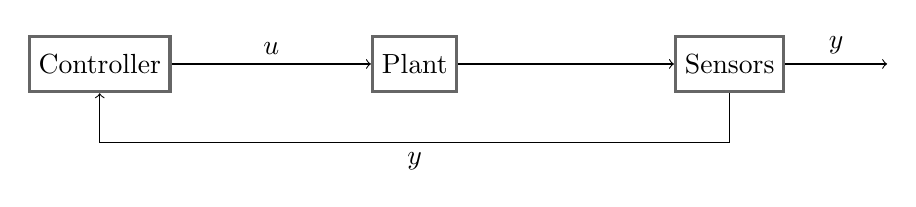
\begin{tikzpicture}[
        block/.style={rectangle, draw=black!60, very thick, minimum size=7mm},
        ]
        \node (plant) at (0,0) [block] {Plant};
        \node (sensors) at (4,0) [block] {Sensors};
        \node (controller) at (-4,0) [block] {Controller};

        \draw[->] (plant) -- (sensors);
        \draw[->] (sensors) -- node[auto] {$y$} (6,0);
        \draw[->] (sensors) -- (4,-1) -- node[auto] {$y$} (-4,-1) -- (controller);
        \draw[->] (controller) -- node[auto] {$u$} (plant);
        
    \end{tikzpicture}
    \caption{Feedback control system}
    \label{fig:feedback-diagram}
\end{figure}
 
\subsection{Observability}
We now aim to reconstruct the full state $x$ from the output $y$ and the input $u$. The following derivation is based on \cite{StephenBoyd2009LectureEstimation}, consider system \eqref{eqn:standard-noiseless-system} where $x$ is unknown and $y$ and $u$ are known. The derivatives of $y$ 
\[
\begin{split}
y &= Cx + Du \\
\dot{y} &= C\dot{x} + Du =  CAx + CBu + D\dot{u} \\
\Ddot{y} &= CA\dot{x} + CBu + Du = CA^{2}x + CABu + CB\dot{u} + D\Ddot{u} \\
\vdots \\
y^{(n_x)} &= CA^{n_x}x + CA^{n_x-1}Bu + CA^{n_x-2}B\dot{u} + \dots + CABu^{(n_x-2)} + CBu^{(n_x-1)} + Du^{(n_x)}
\end{split}
\]
will be used to reconstruct $x$ from the derivatives of $y$ and $u$. These derivatives of $y$ can be combined into
\[ \mathbf{y} =  \mathcal{O}x + \mathcal{K}\mathbf{u}
,\]
where
\[\mathbf{y}=
\begin{bmatrix}
    y \\
    y^{(1)} \\
    y^{(2)} \\
    \vdots \\
    y^{(n-1)} \\
\end{bmatrix} \quad \text{and} \quad
\mathbf{u} = 
\begin{bmatrix}
    u \\
    u^{(1)} \\
    u^{(2)} \\
    \vdots \\
    u^{(n-1)} \\
\end{bmatrix},
\]
are vectors containing the derivatives of the output and the input,
\begin{equation}\label{eqn:observability-matrix}
    \mathcal{O}=
    \begin{bmatrix}
        C \\
        CA \\
        CA^2 \\
        \vdots \\
        CA^{n-1}
    \end{bmatrix}    
\end{equation}

is the \textit{observability matrix} and
\[ \mathcal{K}=
\begin{bmatrix}
    D & 0 & 0 & \hdots & 0\\
    CB & D & 0 & \hdots & 0\\
    CAB & CB & D & \hdots & 0 \\
    \vdots & \vdots & \vdots & \ddots & \vdots \\
    CA^{n-2}B & CA^{n-3}B & CA^{n-4}B & \hdots & D
\end{bmatrix}.
\]
Isolating $x$ results in
\begin{equation}\label{eqn:state-estimation-w-observability-matrix}
    x = \mathcal{O}^{-1}(\mathbf{y}-\mathcal{K}\mathbf{u}).
\end{equation}
As can be seen in \eqref{eqn:state-estimation-w-observability-matrix} observability matrix $\mathcal{O}$ is required to be invertible to reconstruct $x$ from the derivatives of $y$ and $u$. If a system's $A$ and $C$ matrix fulfil this requirement, the system can be described as \textit{observable}. The invertibility requirement is equivalent to the statement that the matrix $\mathcal{O}$ needs to be full rank \cite[Section 2.9]{Lay2016LinearApplications}, this theorem that can also be found in \cite[Corollary 3.8]{Antsaklis2006LinearSystems}. The implication of this is that it is only possible to reconstruct the state $x$ if the pair $(A,C)$ is observable. 

\begin{example}\label{ex:single-ouptut-observability}
    Let us work out an example on the system presented in Example \ref{ex:system} where only the position of the first mass is measured. This leads to the following system matrices:
\begin{equation*}
    A =
    \begin{bmatrix}
        0 & 1 & 0 & 0 \\
        -15 & -2 & 15 & 2 \\
        0 & 0 & 0 & 1 \\
        0 & 0 & -15 & -2 \\
    \end{bmatrix}, \quad
    C =
    \begin{bmatrix}
        1 & 0 & 0 & 0 \\
    \end{bmatrix}.
\end{equation*}
We now compute the observability matrix
\begin{equation*}
    \mathcal{O} = 
    \begin{bmatrix}
        C \\ CA \\ CA^2 \\ CA^3 \\
    \end{bmatrix} =
    \begin{bmatrix}
        1 & 0 & 0 & 0 \\
        0 & 1 & 0 & 0 \\
        -15 & -2 & 15 & 2 \\
        30 & -11 & -60 & 7 \\
    \end{bmatrix}
\end{equation*}
which has rank $4$ and so the pair $(A,C)$ is observable.
\end{example}

Example \ref{ex:single-ouptut-observability} considers a system with only one output, we will now investigate the case with multiple outputs. Let us expand the observability matrix \eqref{eqn:observability-matrix} for a system where $n_y>1$, a system with more than one output.
\begin{equation*}
\mathcal{O}=
\begin{bmatrix}
    C \\
    CA \\
    \vdots \\
    CA^{n-1}
\end{bmatrix}    
=
\begin{bmatrix}
    c_1 \\
    \vdots \\
    c_{n_y} \\
    c_1A \\
    \vdots \\
    c_{n_y}A \\
    \vdots \\
    c_1A^{n-1}\\
    \vdots \\
    c_{n_y}A^{n-1} \\
\end{bmatrix}_{n_xn_y \times n_x}.
\end{equation*}
The same rank condition still holds, the system is fully observable as long as the $\mathcal{O}$ matrix is full rank. This implies that certain combinations of sensors that do not suffice on their own can make a system fully observable \cite[Section 3.4 D 2]{Antsaklis2006LinearSystems}.

\subsection{Single observer}
Let us now reconstruct the full state of system \eqref{eqn:standard-noiseless-system} from  $y$ and $u$ by defining the state estimate as in \cite[Section 16.5]{Hespanha2018LinearTheory}
\begin{equation}\label{eqn:stable-simple-state-estimator}
    \dot{\hat{x}} = A\hat{x} + Bu, \quad \hat{y} = C\hat{x} + Du.
\end{equation}
We now define the \textit{state estimation error}
\begin{equation}\label{eqn:estimate-error}
    e = \hat{x} - x
\end{equation}
which we differentiate and substitute equations \eqref{eqn:standard-noiseless-system} and \eqref{eqn:stable-simple-state-estimator} into to give
\begin{equation*}
    \dot{e} = \dot{\hat{x}} - \dot{x} = A\hat{x} + Bu - Ax - Bu = Ae.
\end{equation*}
We can now conclude that $e \rightarrow 0$ as $t \rightarrow \infty$ if the matrix $A$ is a stability matrix. Let us now define a state estimator that provides an asymptotically correct state estimate even when $A$ is not a stability matrix as in \cite[Section 16.5]{Hespanha2018LinearTheory}:
\begin{equation}\label{eqn:unstable-simple-state-estimator}
    \dot{\hat{x}} = A\hat{x} + Bu + L(\hat{y} - y), \quad \hat{y} = C\hat{x} + Du.
\end{equation}
We now perform the same analysis on the derivative of the state estimation error
\begin{equation}\label{eqn:error-linear-observer}
    \dot{e} = A\hat{x} + Bu + L(C\hat{x} + Du - Cx - Du) - Ax - Bu = (A+LC)e
\end{equation}
which is similar to the solution in \eqref{eqn:zero-input-solution}. From which we can conclude that if $A+LC$ is a stability matrix $e \rightarrow 0$ as $t \rightarrow \infty$. Figure \ref{fig:observer-diagram} shows the observer placed between the sensors and the controller

\begin{figure}[ht]
    \centering
    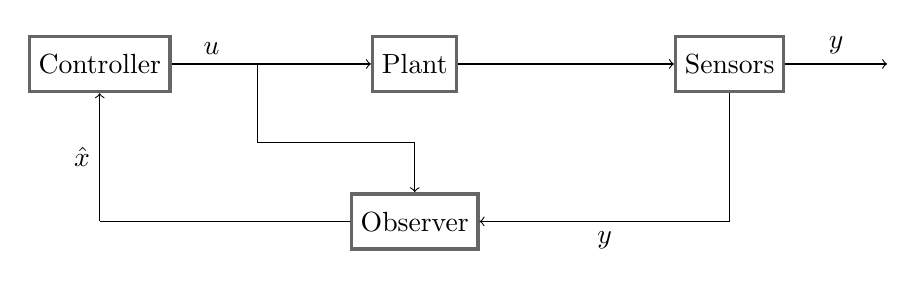
\begin{tikzpicture}[
        block/.style={rectangle, draw=black!60, very thick, minimum size=7mm},
        ]
        \node (plant) at (0,0) [block] {Plant};
        \node (sensors) at (4,0) [block] {Sensors};
        \node (observer) at (0,-2) [block] {Observer};
        \node (controller) at (-4,0) [block] {Controller};

        \draw[->] (plant) -- (sensors);
        \draw[-] (sensors) -- (4,-2);
        \draw[->] (4,-2) -- node[auto] {$y$} (observer);
        \draw[->] (sensors) -- node[auto] {$y$} (6,0);
        \draw[-] (observer)  -- (-4,-2);
        \draw[->] (-4,-2) -- node[auto] {$\hat{x}$} (controller);
        \draw[->] (controller) -- node[pos=0.2,above] {$u$} (plant);
        \draw[->] (-2,0) -- (-2,-1) -- (0,-1) -- (observer);
    \end{tikzpicture}
    \caption{An observer in a control system}
    \label{fig:observer-diagram}
\end{figure}

It is important to note that no restrictions are set on the structure of $y$ and therefore $C$ as long as the pair $(A,C)$ is observable. 

Let us now extend the observer \eqref{eqn:unstable-simple-state-estimator} to also correctly estimate systems with a nonlinear contribution $\phi(x)$. Consider the system
\begin{equation*}\label{eqn:nonlinear-system}
    \dot{x} = Ax + Bu + E\phi(y), \quad y = Cx + Du.
\end{equation*}
The observer will be constructed as
\begin{equation}\label{eqn:nonlinear-single-observer}
    \dot{\hat{x}} = A\hat{x} + Bu + E\phi(y) + L(\hat{y} - y), \quad \hat{y} = C\hat{x} + Du.
\end{equation}
Note that the input to the nonlinearity is $y$. Let us now substitute these definitions into the derivative of the error $e=\hat{x}-x$
\begin{equation*}\label{eqn:errror-nonlinear-observer}
    \begin{split}
        \dot{e} = \dot{\hat{x}} - \dot{x} &= A\hat{x} + Bu + E\phi(y) + L(\hat{y} - y) - Ax - Bu - E\phi(y) \\
        &= (A+LC)e + E(\phi(y) - \phi(y)) \\
        &= (A+LC)e.
    \end{split}
\end{equation*}
It is now evident why $\phi(y)$ is used in equation \eqref{eqn:nonlinear-system}, otherwise $e \rightarrow 0$ as $t \rightarrow \infty$ cannot be guaranteed. Because $\phi(y)$ does not necessarily equal $\phi(x)$, $\phi(y) - \phi(x)$ does not necessarily equal $0$. This does set certain requirements on $y$, variables that affect the nonlinearity need to be measured directly. For the multi mass-spring-damper system as in Chapter \ref{ch:system-definition} this means that all positions $x_a,a=1,2,\dots,b$ need to be measured directly. 

\subsection{Eigenvalue placement}
Since we have full control over $L$, we will now discuss methods to place eigenvalues of $A+LC$ at desired locations and what constraints are limiting our control over these eigenvalues.

\begin{theorem}[Observer eigenvalues]
\label{th:arbitrary-alc-eigenvalues}
    If the pair $(A,C)$\eqref{eqn:standard-noiseless-system} is observable there exists an $L \in \mathbb{R}^{n \times m}$ that influences all eigenvalues of $A+LC$.
\end{theorem}
\begin{proof}
    This proof is based on \cite[Section 4.2]{Antsaklis2006LinearSystems}. Suppose that the pair $(A,C)$ is not fully observable and that all eigenvalues of $A+LC$  have been influenced by $L$, it will be shown that this leads to a contradiction. There exists a similarity transformation that separates the observable from the unobservable part: the observable decomposition \cite[Section 16.1]{Hespanha2018LinearTheory}. Performing this transformation on the pair $(A,C)$ leads to
    \begin{equation}
    \begin{split}
        \begin{bmatrix}
            \dot{x}_o \\
            \dot{x}_u
        \end{bmatrix}
        &=
        \begin{bmatrix}
            A_o & 0 \\
            A_{21} & A_u
        \end{bmatrix}
        \begin{bmatrix}
            x_o \\
            x_u
        \end{bmatrix}
        + 
        \begin{bmatrix}
            L_1 \\
            L_2
        \end{bmatrix}
        \begin{bmatrix}
            C_o & 0
        \end{bmatrix} \\
        &=
        \begin{bmatrix}
            A_o + L_1 C_o & 0 \\
            A_{21} + L_2 C_o & A_u
        \end{bmatrix}
    \end{split}
    \textcolor{red}{equation incomplete}
    \end{equation}  
where the pair $(A_o,C_o)$ is observable. A similarity transformation leaves the eigenvalues unchanged \cite[Section 5.2]{Lay2016LinearApplications}. The lower triangular structure of the matrix implies that the eigenvalues of $A_u$ remain the same, which leads to a contradiction: not all the eigenvalues of $A+LC$ have been influenced. Thus, if the pair $(A,C)$ is observable there exists an $L$ that can influence all eigenvalues of $A+LC$.
\end{proof}

An analytical method to place the eigenvalues at arbitrary locations in a MIMO system is presented in \cite[Section 4.2 B]{Antsaklis2006LinearSystems}, where the system is first transformed into \textit{observer form} by a similarity transformation. After this transformation the deriving the matrix $L$ is convenient. Another option is numerically deriving $L$. Matlab provides the function \texttt{place}, based on the algorithm presented in \cite{Kautsky1985RobustFeedback}.

\textcolor{red}{Unsatisfying conclusion, would prefer to show an actual strategy to choose the eigenvalues.}



\newpage
\input{report/Chapters/4. CMO}
\newpage


\section{State-sharing multi-observer}
In this chapter the state-sharing multi-observer (SSMO) will be discussed, aiming to reduce the required memory to store the CMO. The SSMO described in this chapter will provide the estimates as described in \autoref{subsec:state-estimates} and will employ the same selection procedure as described in \autoref{subsec:estimate-selection}.

\subsection{Constructing the state-estimates}
Let
\begin{equation}\label{eqn:ssmo-observer}
    \begin{split}
        \dot{\hat{x}}_o &= \A_o\hat{x}_o - L_oC_ox + Bu -L_o(v_o + \tau_o), \quad \A_o=A+L_{o}C_{o} \\
    \end{split}
\end{equation}
be a set of observers that contains all $J$- and $P$-observers \eqref{eqn:cmo-single-J-observer}\eqref{eqn:cmo-single-P-observer}, such that $\mcO=\mcJ\bigcup\mcP$ and $o=1,2,\dots,|\mcO|$. All $L_o$ must be selected in such a way that all $\A_o$ share the same characteristic polynomial
\begin{equation}\label{eqn:ssmo-char-poly}
    \det(sI-\A) = p(s) = s^n + q_1s^{n-1} + \dots + q_{n-1}s + q_n
\end{equation}
and thus all have equal eigenvalues. Let us now define a matrix $\Tilde{L}_{o}$ such that $\Tilde{L}_oy=L_oy_o$. This can be achieved by padding $L_o$ with zero vectors $z \in \mathbb{R}^{n \times 1}$ \cite{Chong2023MemoryAlgorithms}. Let us now rewrite the observer \eqref{eqn:ssmo-observer} into the following form
\begin{equation}\label{eqn:ssmo-standard-system-form}
    \dot{\hat{x}}_o = \A_o\hat{x}_o + \B_o\eta_o, \quad
    \B_o =
    \begin{bmatrix}
        E & B & -\Tilde{L}_o \\
    \end{bmatrix}, \quad \eta_o =
    \begin{bmatrix}
        \phi(y) \\
        u \\
        y_o + v_o + \tau_o
    \end{bmatrix}.
\end{equation}

Let us now derive transformation matrices $T_o$ that transform all $\A_o=A+L_{o}C_{o}$ into controllable canonical form as in \cite[Sec. 4.3.2]{Hespanha2018LinearTheory}
\begin{equation}\label{eqn:controllable-canonical-form}
    \mathbf{A} =
    \begin{bmatrix}
        -q_1I_l & -q_2I_l & \cdots & -q_{n-1}I_l & -q_nI_l \\
        I_l & 0_l & \cdots & 0_l & 0_l \\
        0_l & I_l & \cdots & 0_l & 0_l \\
        \vdots & \vdots & \ddots & \vdots & \vdots \\
        0_l & 0_l & \cdots & I_l & 0_l \\
    \end{bmatrix}, \quad
    \mathbf{B} = 
    \begin{bmatrix}
        I_l \\ 0_l \\ \vdots \\ 0_l \\ 0_l \\
    \end{bmatrix}
\end{equation}
where $l=N$. The transformation matrices for each observer are $T_o=R_pR_q$,
\begin{equation}
    \begin{split}
         R_p &=
        \begin{bmatrix}
            \B_o & \A_o\B_o & \A^{2}_o\B_o & \cdots & \A^{n-1}_o\B_o \\
        \end{bmatrix} \\
        R_q &=
        \begin{bmatrix}
            I_l & q_1I_l & q_2I_l & \cdots & q_{n-1}I_l \\
            0_l & I_l & q_1I_l & \cdots & q_{n-2}I_l \\
            \vdots & \ddots & \ddots & \ddots & \vdots \\
            0_l & \cdots & 0_l & I_l & q_1I_l \\
            0_l & \cdots & 0_l & 0_l & I_l \\
        \end{bmatrix}.
    \end{split}
\end{equation}
Let us now show that the following
\begin{equation}\label{eqn:A-transformation}
    \begin{split}
        T_o\mathbf{A} &= \A_oT_o \\
        R_pR_q\mathbf{A} &= \A_oR_pR_q \\
    \end{split}
\end{equation}
holds. Let us start by expanding
\begin{equation*}
    \begin{split}
        R_q\mathbf{A} &=  
        \begin{bmatrix}
            I_l & q_1I_l & q_2I_l & \cdots & q_{n-1}I_l \\
            0_l & I_l & q_1I_l & \cdots & q_{n-2}I_l \\
            \vdots & \ddots & \ddots & \ddots & \vdots \\
            0_l & \cdots & 0_l & I_l & q_1I_l \\
            0_l & \cdots & 0_l & 0_l & I_l \\
        \end{bmatrix}
        \begin{bmatrix}
            -q_1I_l & -q_2I_l & \cdots & -q_{n-1}I_l & -q_nI_l \\
            I_l & 0_l & \cdots & 0_l & 0_l \\
            0_l & I_l & \cdots & 0_l & 0_l \\
            \vdots & \vdots & \ddots & \vdots & \vdots \\
            0_l & 0_l & \cdots & I_l & 0_l \\
        \end{bmatrix} \\
        &= 
        \begin{bmatrix}
            0_l & 0_l & 0_l & \cdots & 0_l & 0_l & 0_l \\
            I_l & q_1I_l & q_2I_l & \cdots & q_{n-3}I_l & q_{n-2}I_l & 0_l \\ 
            0_l & I_l & q_1I_l & \cdots & q_{n-4}I_l & q_{n-3}I_l & 0_l \\ 
            \vdots & \vdots & \vdots & \ddots & \vdots & \vdots & \vdots \\
            0_l & 0_l & 0_l & \cdots & q_1I_l & q_2I_l & 0_l \\
            0_l & 0_l & 0_l & \cdots & I_l & q_1I_l & 0_l \\
            0_l & 0_l & 0_l & \cdots & 0_l & I_l & 0_l \\
        \end{bmatrix}.
    \end{split} 
\end{equation*}
We now premultiply this by $R_o$
\begin{equation*}
    \begin{split}
        R_pR_q\mathbf{A} &= 
        \begin{bmatrix}
            \B_o & \A_o\B_o & \A^{2}_o\B_o & \cdots & \A^{n-1}_o\B_o \\
        \end{bmatrix}
        \begin{bmatrix}
            0_l & 0_l & 0_l & \cdots & 0_l & 0_l \\
            I_l & q_1I_l & q_2I_l & \cdots & q_{n-2}I_l & 0_l \\ 
            0_l & I_l & q_1I_l & \cdots & q_{n-3}I_l & 0_l \\ 
            \vdots & \ddots & \ddots & \ddots & \vdots & \vdots \\
            0_l & 0_l & 0_l & \ddots & q_1I_l & 0_l \\
            0_l & 0_l & 0_l & \cdots & I_l & 0_l \\
        \end{bmatrix} \\
        &= 
        \begin{bmatrix}
            \A_o\B_o \\ q_1\A_o\B_o + \A^2_o\B_o \\ q_2\A_o\B_o + q_1\A^2_o\B_o + \A^3_o\B_o \\ \cdots \\ q_{n-2}\A_o\B_o + q_{n-3}\A^2_o\B_o + \cdots + q_1\A^{n-2}_o\B_o + \A^{n-1}_o\B_o \\ 0 \\      
        \end{bmatrix}^T
    \end{split}
\end{equation*}
Where by the Cayley-Hamilton theorem we can rewrite penultimate column as
\begin{equation*}
    \begin{bmatrix}
            \A_o\B_o \\ q_1\A_o\B_o + \A^2_o\B_o \\ q_2\A_o\B_o + q_1\A^2_o\B_o + \A^3_o\B_o \\ \vdots \\ -\A^n_o\B_o \\ 0 \\      
        \end{bmatrix}^T
\end{equation*}

We now expand
\begin{equation*}
    \begin{split}
        \A_oR_pR_q &= 
        \begin{bmatrix}
            \A_o\B_o & \A^2_o\B_o & \A^{3}_o\B_o & \cdots & \A^{n}_o\B_o \\
        \end{bmatrix}
        \begin{bmatrix}
            I_l & q_1I_l & q_2I_l & \cdots & q_{n-1}I_l \\
            0_l & I_l & q_1I_l & \cdots & q_{n-2}I_l \\
            \vdots & \ddots & \ddots & \ddots & \vdots \\
            0_l & \cdots & 0_l & I_l & q_1I_l \\
            0_l & \cdots & 0_l & 0_l & I_l \\
        \end{bmatrix} \\
        &=
        \begin{bmatrix}
            \A_o\B_o \\ 
            q_1\A_o\B_o + \A^2_o\B_o \\ 
            q_2\A_o\B_o + q_1\A^2\B_o + \A^3_o\B_o \\ \vdots \\ 
            q_{n-1}\A_o\B_o + q_{n-2}\A^2_o\B_o + \cdots + \A^{n-1}_o\B_o \\
            q_{n-1}\A_o\B_o + q_{n-2}\A^2_o\B_o + \cdots + \A^{n-1}_o\B_o + \A^n_o\B_o \\
        \end{bmatrix}^T,
    \end{split}
\end{equation*}
where the bottom two rows can be simplified by using the Cayley-Hamilton theorem
\begin{equation*}
    \begin{split}
        \A_oR_pR_q &= 
        \begin{bmatrix}
            \A_o\B_o \\ 
            q_1\A_o\B_o + \A^2_o\B_o \\ 
            q_2\A_o\B_o + q_1\A^2\B_o + \A^3_o\B_o \\ \vdots \\ 
            \A^{n}_o\B_o \\
            0 \\
        \end{bmatrix}^T,
    \end{split}
\end{equation*}
which is equal to $R_oR_q\A_o$. We can now conclude that the matrix $T_o=R_oR_q$ satisfies \eqref{eqn:A-transformation}. Now we will show the same for
\begin{equation}\label{eqn:B-transformation}
    \begin{split}
        T_o\mathbf{B} &= \B_o \\
        R_pR_q\mathbf{B} &= \B_o.
    \end{split}
\end{equation}
Let us expand
\begin{equation*}
    \begin{split}
        R_pR_q\mathbf{B} &=
        \begin{bmatrix}
            \B_o & \A_o\B_o & \A^{2}_o\B_o & \cdots & \A^{n-1}_o\B_o \\
        \end{bmatrix}
        \begin{bmatrix}
            I_l & q_1I_l & q_2I_l & \cdots & q_{n-1}I_l \\
            0_l & I_l & q_1I_l & \cdots & q_{n-2}I_l \\
            \vdots & \ddots & \ddots & \ddots & \vdots \\
            0_l & \cdots & 0_l & I_l & q_1I_l \\
            0_l & \cdots & 0_l & 0_l & I_l \\
        \end{bmatrix}
        \begin{bmatrix}
            I_l \\ 0_l \\ \vdots \\ 0_l \\ 0_l \\
        \end{bmatrix} \\
        &=
        \begin{bmatrix}
            \B_o & \A_o\B_o & \A^{2}_o\B_o & \cdots & \A^{n-1}_o\B_o \\
        \end{bmatrix}
        \begin{bmatrix}
            I_l \\ 0_l \\ \vdots \\ 0_l \\ 0_l \\
        \end{bmatrix} = \B_o \\
    \end{split}
\end{equation*}
which shows that \eqref{eqn:B-transformation} holds. It should be noted that $\mathbf{A}$ and $\mathbf{B}$ are independent of $o$ and since all observers \eqref{eqn:ssmo-observer} share the same characteristic polynomial \eqref{eqn:ssmo-char-poly}, $\mathbf{A}$ and $\mathbf{B}$ are the same for all observers. This means that only one copy of the matrices needs to be stored and all state estimates $\hat{x}$ from the transformation matrices.

\subsection{Implementation}
Let us set the initial conditions of all state estimates to be equal, we will choose $0$ for simplicity. When all initial conditions are zero $z$ will also be the same for all state estimates, 
\begin{equation*}
    \dot{z} = \mathbf{A}z + \mathbf{B}\eta, \quad \eta = 
    \begin{bmatrix}
        u \\ y + v + \tau
    \end{bmatrix}.
\end{equation*}
We then transform $z$ into the original state estimates by

\begin{equation*}
    \tilde{x}_{SSMO} = \texttt{pm}(T,z,3),
\end{equation*}
where
\begin{center}
    % \begin{minipage}[t]{0.4\textwidth}
    %     \centering
    %     % first tikzpicture
    %     \begin{equation*}
    %         \begin{tikzpicture}[every node/.style={anchor=north east,fill=white,minimum width=1.2cm,minimum height=7mm}]
            
    %         % Define the displacement as a coordinate
    %         \coordinate (displacement) at (0.9,0.2);
        
    %         \matrix (mLP) [draw,matrix of math nodes]
    %             {
    %             \hat{x}_{\cP}^\mcJ \\
    %             };
        
    %         \matrix (dots2) [draw,matrix of math nodes] at ($(mLP.south west)+(displacement)$)
    %             {
    %             \dots \\
    %             };
        
    %         \matrix (mLp) [draw,matrix of math nodes] at ($(dots2.south west)+(displacement)$)
    %             {
    %             \hat{x}_{1}^\mcP \\
    %             };
        
    %         \matrix (mLJ) [draw,matrix of math nodes] at ($(mLp.south west)+(displacement)$)
    %             {
    %             \hat{x}_{\cJ}^\mcJ \\
    %             };
        
    %         \matrix (dots1) [draw,matrix of math nodes] at ($(mLJ.south west)+(displacement)$)
    %             {
    %             \dots \\
    %             };
        
    %         \matrix (mLj) [draw,matrix of math nodes] at ($(dots1.south west)+(displacement)$)
    %             {
    %             \hat{x}_1^\mcJ \\
    %             };
            
    %         \draw[dashed](mLj.north east)--(mLP.north east);
    %         \draw[dashed](mLj.north west)--(mLP.north west);
    %         \draw[dashed](mLj.south east)--(mLP.south east);
            
    %         \node at ($(-4,-1.8)$) {$\hat{x}_{SSMO}=$};
            
    %         \end{tikzpicture}
    %     \end{equation*}
    % \end{minipage}
    \begin{minipage}[t]{0.4\textwidth}
    \centering
    % Second tikzpicture
        \begin{equation}
            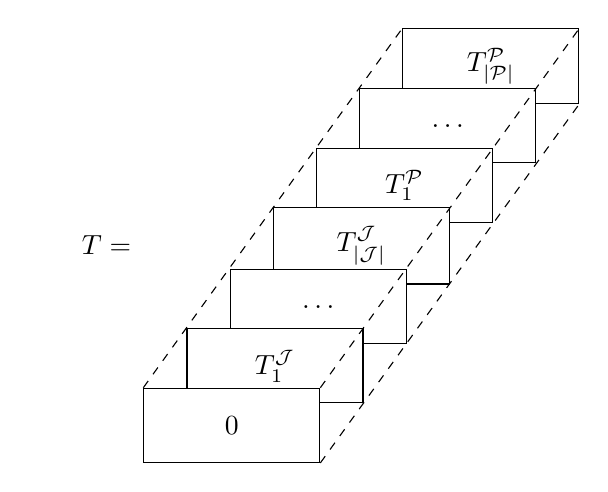
\begin{tikzpicture}[every node/.style={anchor=north east,fill=white,minimum width=2cm,minimum height=7mm}]
            
            % Define the displacement as a coordinate
            \coordinate (displacement) at (1.7,0.2);
        
            \matrix (mLP) [draw,matrix of math nodes]
                {
                T^\mcP_{|\mcP|} \\
                };
        
            \matrix (dots2) [draw,matrix of math nodes] at ($(mLP.south west)+(displacement)$)
                {
                \dots \\
                };
        
            \matrix (mLp) [draw,matrix of math nodes] at ($(dots2.south west)+(displacement)$)
                {
                T^\mcP_{1} \\
                };
        
            \matrix (mLJ) [draw,matrix of math nodes] at ($(mLp.south west)+(displacement)$)
                {
                T^\mcJ_{|\mcJ|} \\
                };
        
            \matrix (dots1) [draw,matrix of math nodes] at ($(mLJ.south west)+(displacement)$)
                {
                \dots \\
                };
        
            \matrix (mLj) [draw,matrix of math nodes] at ($(dots1.south west)+(displacement)$)
                {
                T^\mcJ_1 \\
                };

            \matrix (m0) [draw,matrix of math nodes] at ($(mLj.south west)+(displacement)$)
                {
                0 \\
                };
            
            \draw[dashed](m0.north east)--(mLP.north east);
            \draw[dashed](m0.north west)--(mLP.north west);
            \draw[dashed](m0.south east)--(mLP.south east);
            
            \node at ($(-5,-2.4)$) {$T=$};
            
            \end{tikzpicture}
        \end{equation}
    \end{minipage}
\end{center}
The structure of the storage matrix $\tilde{x}_{SSMO}$ is the same as $\tilde{x}_{3D}$ in \eqref{eqn:A-tilde-3D}. The selection of the final estimate follows the same procedure as described in Section \ref{subsec:estimate-selection}.

\begin{table}[h]
    \centering
    \begin{tabular}{c|c|c}
       Matrix  & Dimensions & Number of elements \\ \hline
       $\Tilde{x}_{SSMO}$  & $ n \times 1 \times N_S$ & $nN_S$ \\
       $\mathbf{A}$ & $nN \times nN$ & $n^2N^2$ \\ 
       $\mathbf{B}$ & $nN \times n$ & $n^2N$ \\
       $T$ & $n \times nN \times N_S$ & $n^2NN_S$ \\
    \end{tabular}
    \caption{SSMO system matrix dimensions}
    \label{tab:SSMO-dimensions}
\end{table}

\subsection{Size comparison}
\newpage
\section{Matlab implementation}\label{ch:matlab-implementation}
Both CMOs and the SSMO as defined in Subsections \ref{subsec:CMO-architecture} and \ref{subsec:ssmo-architecture} have been implemented in Matlab. In this chapter the implementations will be discussed and the MOs will be applied on the mass-spring-damper system as described in Chapter \ref{ch:system-definition}. The implementation uses classes for the system, attack, shared multi-observers and the specific multi-observers. All of these will be discussed in this chapter, the code itself can be found in Appendix \ref{ap:matlab-code}.

\subsection{Class explanation}
The system class (\texttt{msd}) defines the system matrices for a mass-spring-damper as in Chapter \ref{ch:system-definition}. The class can creates the state-space system consisting of matrices \eqref{eqn:msd-A}\eqref{eqn:msd-B}\eqref{eqn:msd-E}\eqref{eqn:msd-C}. The class can create both linear and nonlinear systems and works for any number of masses in series.

The \texttt{attack} class defines an attack on the system, the outputs that are to be attacked can be specified. If no outputs are specified, a random selection is made. A list with ones indicating an attack and zeros indicating no attack is made, later on this one is substituted by the attack signal. The specific attack signal can be changed within the \texttt{attackFunction} function.

All MOs are based on a common set of $J$-observers and $P$-observers as defined in Subsection \ref{subsec:state-estimates}. Since all MOs observe the same system, these observers can be defined once and used by all MOs. A separate \texttt{mo} object needs to be generated for both the $J$ and $P$-observers. The \texttt{mo} defines observers for each combination as defined in \eqref{eqn:observer-sets}, based on a given number of outputs for each observer (size of each combination). The class generates an $L$ matrix that places the eigenvalues of $A + LC$ at specified locations. Usually, the size of $C$ does not match the number of outputs $N_O$. The \texttt{mo} class automatically creates a set of outputs based on the provided $C$ where the number of rows matches $N_O$.

The \texttt{cmo2d} class defines the 2D CMO based on the two \texttt{mo} objects for the $J$ and $P$-observers and the system.  It constructs the system matrices as in \eqref{eqn:2D-CMO} and defines the 2D attack vector for use on the 2D CMO.

The \texttt{cmo3d} class defines the 3D CMO based on the two \texttt{mo} objects. It generates the system matrices \eqref{eqn:x3d},\eqref{eqn:A-tilde-3D},\eqref{eqn:F-3d}\eqref{eqn:L-3d} and \eqref{eqn:eta-3d} and uses the \texttt{attack} object to create a 3D attack vector that stores the ones and zeros for each specific observer.

The \texttt{ssmo} class defines the SSMO based on the \texttt{mo} objects. It generates the shared system matrices \eqref{eqn:controllable-canonical-form} and all transformation matrices \eqref{eqn:ssmo-transformation}. 

\subsection{Running a simulation}
All MOs can be simulated under the same conditions and the results can be compared. The file \texttt{mainClassScript.m} in Appendix \ref{ap:matlab-code}, generates all MOs and solves the ODEs as in equation \eqref{eqn:standard-system}, \eqref{eqn:cmo-single-J-observer} and \eqref{eqn:cmo-single-P-observer}. Figure \ref{fig:unattacked-system-plot} displays the solution of this ODE for the system as in Example \ref{ex:system}. The observer quickly approaches the system state and the error decays to zero.

\newpage
\begin{figure}[H]
    \centering
    \includegraphics[width=\linewidth]{report/Figures/symplot_5o0a.png}
    \caption{An unattacked, noiseless double mass-spring-damper system and an observer.}
    \label{fig:unattacked-system-plot}
\end{figure}

Let us now introduce the attack as in Figure \ref{fig:attack-diagram}, so outputs $2$ and $5$ are under attack. The attack signal $\tau_j=t,j=2,5$ is injected into both outputs. Figure \ref{fig:attacked-system-plot} shows the result of such an attack, all but one of the red dashed $J$-estimates diverge from the actual state (the one that converges overlaps with the light blue line). The MO is able to correctly select the correct state estimate from the observer that uses the outputs $1,3$ and $4$ to construct its state estimate. The blue dashed lines show the $P$-estimators, each constructed with a single output. In this case three of them converge and the other two diverge. 
\newpage
\begin{figure}[H]
    \centering
    \includegraphics[width=\linewidth]{report/Figures/symplot_5o2a}
    \caption{An attacked noiseless double mass-spring-damper system and a multi-observer. Outputs 2 and 5 are under attack with attack signal $\tau=t$.} 
    \label{fig:attacked-system-plot}
\end{figure}

\textcolor{red}{todo
\begin{itemize}
    \item noise
    \item simulate different attacks
\end{itemize}
}

\newpage
\bibliographystyle{plain}
\bibliography{report/references.bib}

\newpage
\begin{appendices}

\section{Stirling's approximation}
\begin{table}[ht]
\centering
\begin{tabular}{|c|c|c|}
\toprule
\textbf{n} & \textbf{Exact Factorial} & \textbf{Stirling's Approximation} \\ \midrule
1 & $1$ & $0.9221$ \\
2 & $2$ & $1.9190$ \\
3 & $6$ & $5.8362$ \\
4 & $24$ & $23.5062$ \\
5 & $120$ & $118.0192$ \\
6 & $720$ & $710.0782$ \\
7 & $5040$ & $4.9804 \times 10^3$ \\
8 & $40320$ & $3.9902 \times 10^4$ \\
9 & $362880$ & $3.5954 \times 10^5$ \\
10 & $3628800$ & $3.5987 \times 10^6$ \\
11 & $39916800$ & $3.9616 \times 10^7$ \\
12 & $479001600$ & $4.7569 \times 10^8$ \\
13 & $6.2270 \times 10^9$ & $6.1872 \times 10^9$ \\
14 & $8.7178 \times 10^{10}$ & $8.6661 \times 10^{10}$ \\
15 & $1.3077 \times 10^{12}$ & $1.3004 \times 10^{12}$ \\
16 & $2.0923 \times 10^{13}$ & $2.0814 \times 10^{13}$ \\
17 & $3.5569 \times 10^{14}$ & $3.5395 \times 10^{14}$ \\
18 & $6.4024 \times 10^{15}$ & $6.3728 \times 10^{15}$ \\
19 & $1.2165 \times 10^{17}$ & $1.2111 \times 10^{17}$ \\
20 & $2.4329 \times 10^{18}$ & $2.4228 \times 10^{18}$ \\
\bottomrule
\end{tabular}
\caption{Comparison of Exact Factorial and Stirling's Approximation}
\label{tab:factorial_stirling}
\end{table}

\section{SSMO transformation matrix}\label{ap:ssmo-transformation-matrix}
Let us now show that the transformation matrix $T_o=R_pR_q$,
\begin{equation*}
    \begin{split}
         R_p &=
        \begin{bmatrix}
            \B_o & \A_o\B_o & \A^{2}_o\B_o & \cdots & \A^{n-1}_o\B_o \\
        \end{bmatrix} \\
        R_q &=
        \begin{bmatrix}
            I_l & q_1I_l & q_2I_l & \cdots & q_{n-1}I_l \\
            0_l & I_l & q_1I_l & \cdots & q_{n-2}I_l \\
            \vdots & \ddots & \ddots & \ddots & \vdots \\
            0_l & \cdots & 0_l & I_l & q_1I_l \\
            0_l & \cdots & 0_l & 0_l & I_l \\
        \end{bmatrix}.
    \end{split}
\end{equation*}
transforms the system \eqref{eqn:ssmo-standard-system-form} into controllable canonical form as in Equation \eqref{eqn:controllable-canonical-form}, with the transformation
\begin{equation}\label{eqn:A-transformation}
    \begin{split}
        T_o\mathbf{A} &= \A_oT_o \\
        R_pR_q\mathbf{A} &= \A_oR_pR_q. \\
    \end{split}
\end{equation}
 Let us start by expanding
\begin{equation*}
    \begin{split}
        R_q\mathbf{A} &=  
        \begin{bmatrix}
            I_l & q_1I_l & q_2I_l & \cdots & q_{n-1}I_l \\
            0_l & I_l & q_1I_l & \cdots & q_{n-2}I_l \\
            \vdots & \ddots & \ddots & \ddots & \vdots \\
            0_l & \cdots & 0_l & I_l & q_1I_l \\
            0_l & \cdots & 0_l & 0_l & I_l \\
        \end{bmatrix}
        \begin{bmatrix}
            -q_1I_l & -q_2I_l & \cdots & -q_{n-1}I_l & -q_nI_l \\
            I_l & 0_l & \cdots & 0_l & 0_l \\
            0_l & I_l & \cdots & 0_l & 0_l \\
            \vdots & \vdots & \ddots & \vdots & \vdots \\
            0_l & 0_l & \cdots & I_l & 0_l \\
        \end{bmatrix} \\
        &= 
        \begin{bmatrix}
            0_l & 0_l & 0_l & \cdots & 0_l & 0_l & 0_l \\
            I_l & q_1I_l & q_2I_l & \cdots & q_{n-3}I_l & q_{n-2}I_l & 0_l \\ 
            0_l & I_l & q_1I_l & \cdots & q_{n-4}I_l & q_{n-3}I_l & 0_l \\ 
            \vdots & \vdots & \vdots & \ddots & \vdots & \vdots & \vdots \\
            0_l & 0_l & 0_l & \cdots & q_1I_l & q_2I_l & 0_l \\
            0_l & 0_l & 0_l & \cdots & I_l & q_1I_l & 0_l \\
            0_l & 0_l & 0_l & \cdots & 0_l & I_l & 0_l \\
        \end{bmatrix}.
    \end{split} 
\end{equation*}
We now premultiply this by $R_o$
\begin{equation*}
    \begin{split}
        R_pR_q\mathbf{A} &= 
        \begin{bmatrix}
            \B_o & \A_o\B_o & \A^{2}_o\B_o & \cdots & \A^{n-1}_o\B_o \\
        \end{bmatrix}
        \begin{bmatrix}
            0_l & 0_l & 0_l & \cdots & 0_l & 0_l \\
            I_l & q_1I_l & q_2I_l & \cdots & q_{n-2}I_l & 0_l \\ 
            0_l & I_l & q_1I_l & \cdots & q_{n-3}I_l & 0_l \\ 
            \vdots & \ddots & \ddots & \ddots & \vdots & \vdots \\
            0_l & 0_l & 0_l & \ddots & q_1I_l & 0_l \\
            0_l & 0_l & 0_l & \cdots & I_l & 0_l \\
        \end{bmatrix} \\
        &= 
        \begin{bmatrix}
            \A_o\B_o \\ q_1\A_o\B_o + \A^2_o\B_o \\ q_2\A_o\B_o + q_1\A^2_o\B_o + \A^3_o\B_o \\ \cdots \\ q_{n-2}\A_o\B_o + q_{n-3}\A^2_o\B_o + \cdots + q_1\A^{n-2}_o\B_o + \A^{n-1}_o\B_o \\ 0 \\      
        \end{bmatrix}^T
    \end{split}
\end{equation*}
Where by the Cayley-Hamilton theorem we can rewrite penultimate column as
\begin{equation*}
    \begin{bmatrix}
            \A_o\B_o \\ q_1\A_o\B_o + \A^2_o\B_o \\ q_2\A_o\B_o + q_1\A^2_o\B_o + \A^3_o\B_o \\ \vdots \\ -\A^n_o\B_o \\ 0 \\      
        \end{bmatrix}^T
\end{equation*}

We now expand
\begin{equation*}
    \begin{split}
        \A_oR_pR_q &= 
        \begin{bmatrix}
            \A_o\B_o & \A^2_o\B_o & \A^{3}_o\B_o & \cdots & \A^{n}_o\B_o \\
        \end{bmatrix}
        \begin{bmatrix}
            I_l & q_1I_l & q_2I_l & \cdots & q_{n-1}I_l \\
            0_l & I_l & q_1I_l & \cdots & q_{n-2}I_l \\
            \vdots & \ddots & \ddots & \ddots & \vdots \\
            0_l & \cdots & 0_l & I_l & q_1I_l \\
            0_l & \cdots & 0_l & 0_l & I_l \\
        \end{bmatrix} \\
        &=
        \begin{bmatrix}
            \A_o\B_o \\ 
            q_1\A_o\B_o + \A^2_o\B_o \\ 
            q_2\A_o\B_o + q_1\A^2\B_o + \A^3_o\B_o \\ \vdots \\ 
            q_{n-1}\A_o\B_o + q_{n-2}\A^2_o\B_o + \cdots + \A^{n-1}_o\B_o \\
            q_{n-1}\A_o\B_o + q_{n-2}\A^2_o\B_o + \cdots + \A^{n-1}_o\B_o + \A^n_o\B_o \\
        \end{bmatrix}^T,
    \end{split}
\end{equation*}
where the bottom two rows can be simplified by using the Cayley-Hamilton theorem
\begin{equation*}
    \begin{split}
        \A_oR_pR_q &= 
        \begin{bmatrix}
            \A_o\B_o \\ 
            q_1\A_o\B_o + \A^2_o\B_o \\ 
            q_2\A_o\B_o + q_1\A^2\B_o + \A^3_o\B_o \\ \vdots \\ 
            \A^{n}_o\B_o \\
            0 \\
        \end{bmatrix}^T,
    \end{split}
\end{equation*}
which is equal to $R_oR_q\A_o$. We can now conclude that the matrix $T_o=R_oR_q$ satisfies \eqref{eqn:A-transformation}. Now we will show the same for
\begin{equation}\label{eqn:B-transformation}
    \begin{split}
        T_o\mathbf{B} &= \B_o \\
        R_pR_q\mathbf{B} &= \B_o.
    \end{split}
\end{equation}
Let us expand
\begin{equation*}
    \begin{split}
        R_pR_q\mathbf{B} &=
        \begin{bmatrix}
            \B_o & \A_o\B_o & \A^{2}_o\B_o & \cdots & \A^{n-1}_o\B_o \\
        \end{bmatrix}
        \begin{bmatrix}
            I_l & q_1I_l & q_2I_l & \cdots & q_{n-1}I_l \\
            0_l & I_l & q_1I_l & \cdots & q_{n-2}I_l \\
            \vdots & \ddots & \ddots & \ddots & \vdots \\
            0_l & \cdots & 0_l & I_l & q_1I_l \\
            0_l & \cdots & 0_l & 0_l & I_l \\
        \end{bmatrix}
        \begin{bmatrix}
            I_l \\ 0_l \\ \vdots \\ 0_l \\ 0_l \\
        \end{bmatrix} \\
        &=
        \begin{bmatrix}
            \B_o & \A_o\B_o & \A^{2}_o\B_o & \cdots & \A^{n-1}_o\B_o \\
        \end{bmatrix}
        \begin{bmatrix}
            I_l \\ 0_l \\ \vdots \\ 0_l \\ 0_l \\
        \end{bmatrix} = \B_o \\
    \end{split}
\end{equation*}
which shows that \eqref{eqn:B-transformation} holds.

\section{Matlab code Chapter \ref{ch:standard-observer}}
\lstinputlisting[style=Matlab-editor,caption=jordan_form.m]{conventional/jordan_form.m}

\section{Matlab code Chapter \ref{ch:cmo}}
\lstinputlisting[style=Matlab-editor,caption=sizeComparison.m]{conventional/sizeComparison.m}
    
\section{Matlab code Chapter \ref{ch:matlab-implementation}}\label{ap:matlab-code}
Firstly, the main scripts is shown. This is the script than should be executed to run the model. Secondly, all classes are shown and finally all functions are shown. The documentation that sits between the function definitions and the start of the code are made by inputting the full function into ChatGPT-4 and with the prompt: "Can you provide documentation for this function? $<$code in between these brackets$>$" All output has been checked and corrected by the author in this report, so that the documentation accurately describes the code.
\lstinputlisting[style=Matlab-editor,caption=mainClassScript.m]{conventional/mainClassScript.m}
Now all classes follow alphabetically
\lstinputlisting[style=Matlab-editor,caption=attack.m]{functions/attack.m}
\lstinputlisting[style=Matlab-editor,caption=cmo2d.m]{functions/cmo2d.m}
\lstinputlisting[style=Matlab-editor,caption=cmo3d.m]{functions/cmo3d.m}
\lstinputlisting[style=Matlab-editor,caption=ssmo.m]{functions/ssmo.m}
\lstinputlisting[style=Matlab-editor,caption=mo.m]{functions/mo.m}
\lstinputlisting[style=Matlab-editor,caption=msd.m]{functions/msd.m}

Now all functions follow alphabetically
\lstinputlisting[style=Matlab-editor,caption=ApLCSetup.m]{functions/ApLCSetup.m}
\lstinputlisting[style=Matlab-editor,caption=attackFunction.m]{functions/attackFunction.m}
\lstinputlisting[style=Matlab-editor,caption=CNSetup.m]{functions/CNSetup.m}
\lstinputlisting[style=Matlab-editor,caption=CsetSetup.m]{functions/Csetsetup.m}
\lstinputlisting[style=Matlab-editor,caption=defineObservers.m]{functions/defineObservers.m}
\lstinputlisting[style=Matlab-editor,caption=etaSetup.m]{functions/etaSetup.m}
\lstinputlisting[style=Matlab-editor,caption=findIndices.m]{functions/findIndices.m}
\lstinputlisting[style=Matlab-editor,caption=flatten.m]{functions/flatten.m}
\lstinputlisting[style=Matlab-editor,caption=generateCombination.m]{functions/generateCombination.m}
\lstinputlisting[style=Matlab-editor,caption=inputDialog.m]{functions/inputDialog.m}
\lstinputlisting[style=Matlab-editor,caption=isMatrixStable.m]{functions/isMatrixStable.m}
\lstinputlisting[style=Matlab-editor,caption=isMemberOf.m]{functions/isMemberOf.m}
\lstinputlisting[style=Matlab-editor,caption=isObsv.m]{functions/isObsv.m}
\lstinputlisting[style=Matlab-editor,caption=isSubsetOf.m]{functions/isSubsetOf.m}
\lstinputlisting[style=Matlab-editor,caption=MOplot.m]{functions/MOplot.m}
\lstinputlisting[style=Matlab-editor,caption=multiObserverODE]{functions/multiObserverODE.m}
\lstinputlisting[style=Matlab-editor,caption=NLspring.m]{functions/NLspring.m}
\lstinputlisting[style=Matlab-editor,caption=pad3DL.m]{functions/pad3DL.m}
\lstinputlisting[style=Matlab-editor,caption=padL.m]{functions/padL.m}
\lstinputlisting[style=Matlab-editor,caption=rootsToCoefficients.m]{functions/rootsToCoefficients.m}
\lstinputlisting[style=Matlab-editor,caption=selectBestEstimate.m]{functions/selectBestEstimate.m}
\lstinputlisting[style=Matlab-editor,caption=selectRandomSubset.m]{functions/selectRandomSubset.m}
\lstinputlisting[style=Matlab-editor,caption=SSMOTransformationSetup.m]{functions/SSMOTransformationSetup.m}
\lstinputlisting[style=Matlab-editor,caption=systemPSetup.m]{functions/systemPSetup.m}
\lstinputlisting[style=Matlab-editor,caption=x0setup.m]{functions/x0setup.m}

\end{appendices}

\end{document}

